\documentclass{article}
\usepackage[utf8]{inputenc}
\usepackage{graphicx}
\usepackage[margin=0.6in]{geometry}
\graphicspath{ {images/} }


\title{Wireless lab week 1}
\author{Steven "Steven"}
\date{February 2017}

\begin{document}

\maketitle


\section{Introduction}

The purpose of this week's lab session is to prepare your PC / laptop with Android Studio. We will require android studio configured before week 2. Android studio can be downloaded for Windows / OSX / Linux. This week, we will try to create a hello world application to make sure everything is configured correctly.


\section{Follow these steps after installing android studio}

\subsection{Create new project}

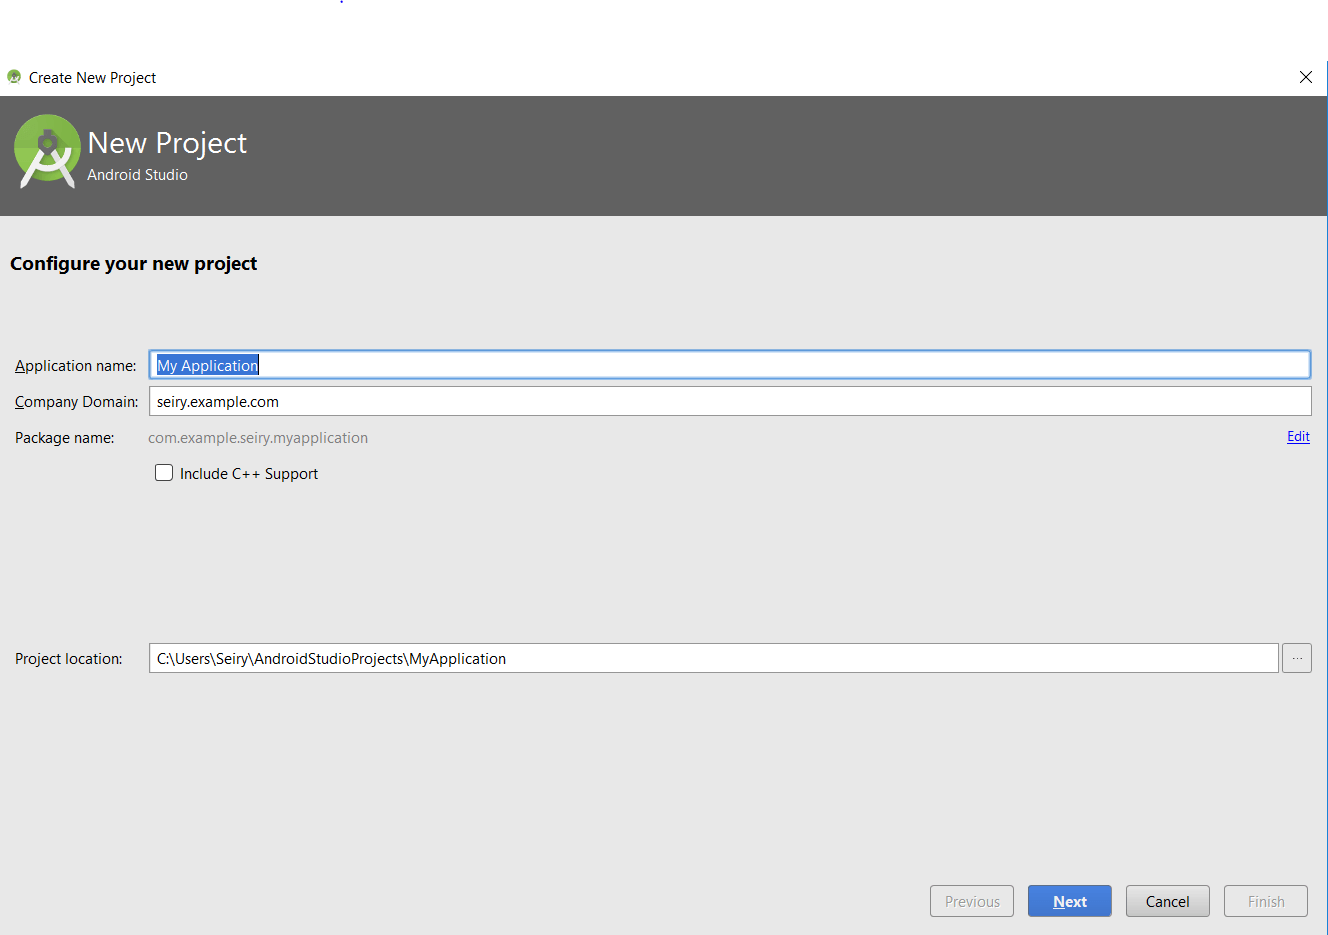
\includegraphics[width=\textwidth]{lab1-1}

\subsection{Choose target ~ Jelly beans is a good target}

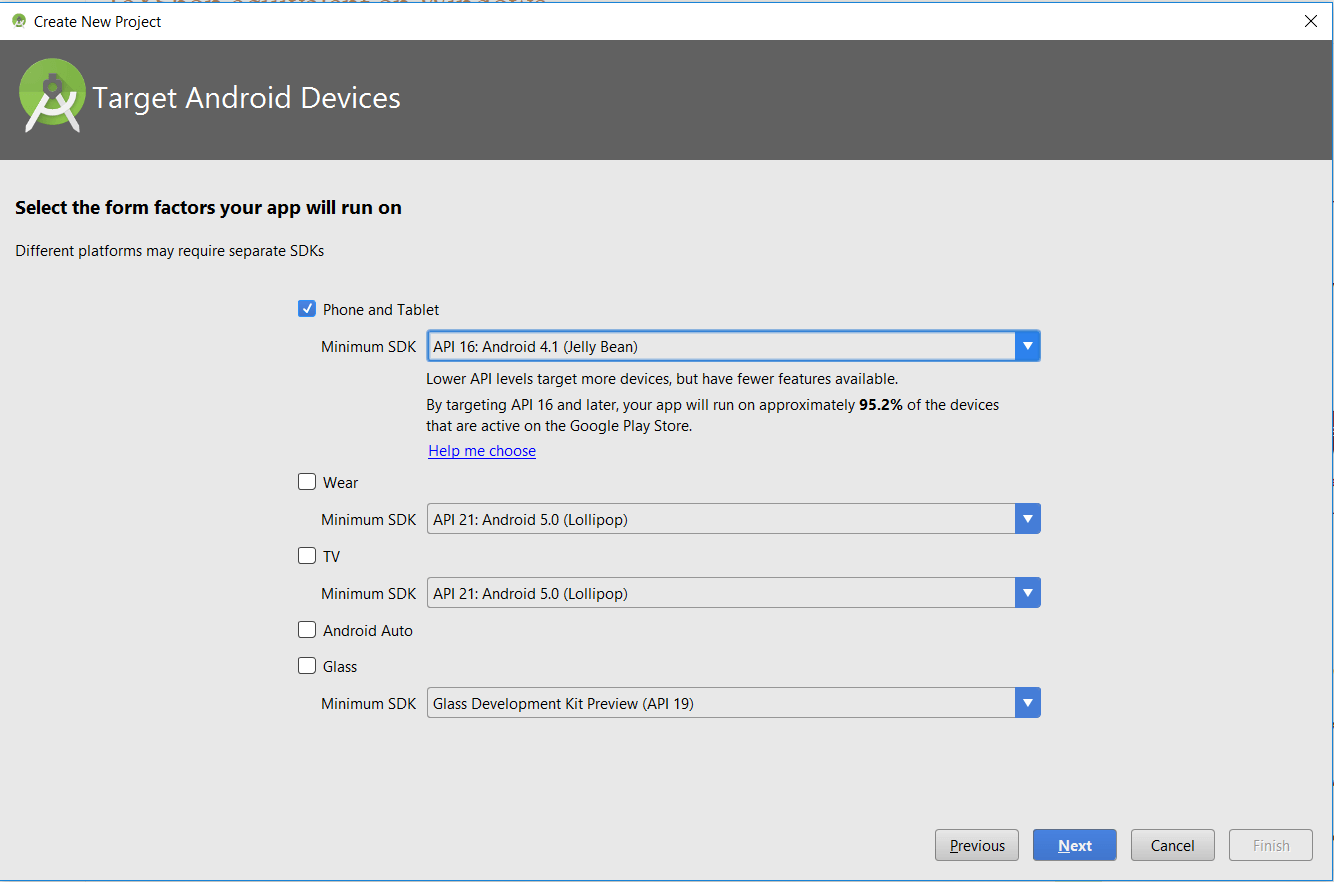
\includegraphics[width=\textwidth]{lab1-2}

\subsection{Choose root activity for the application. For now choose empty activity}

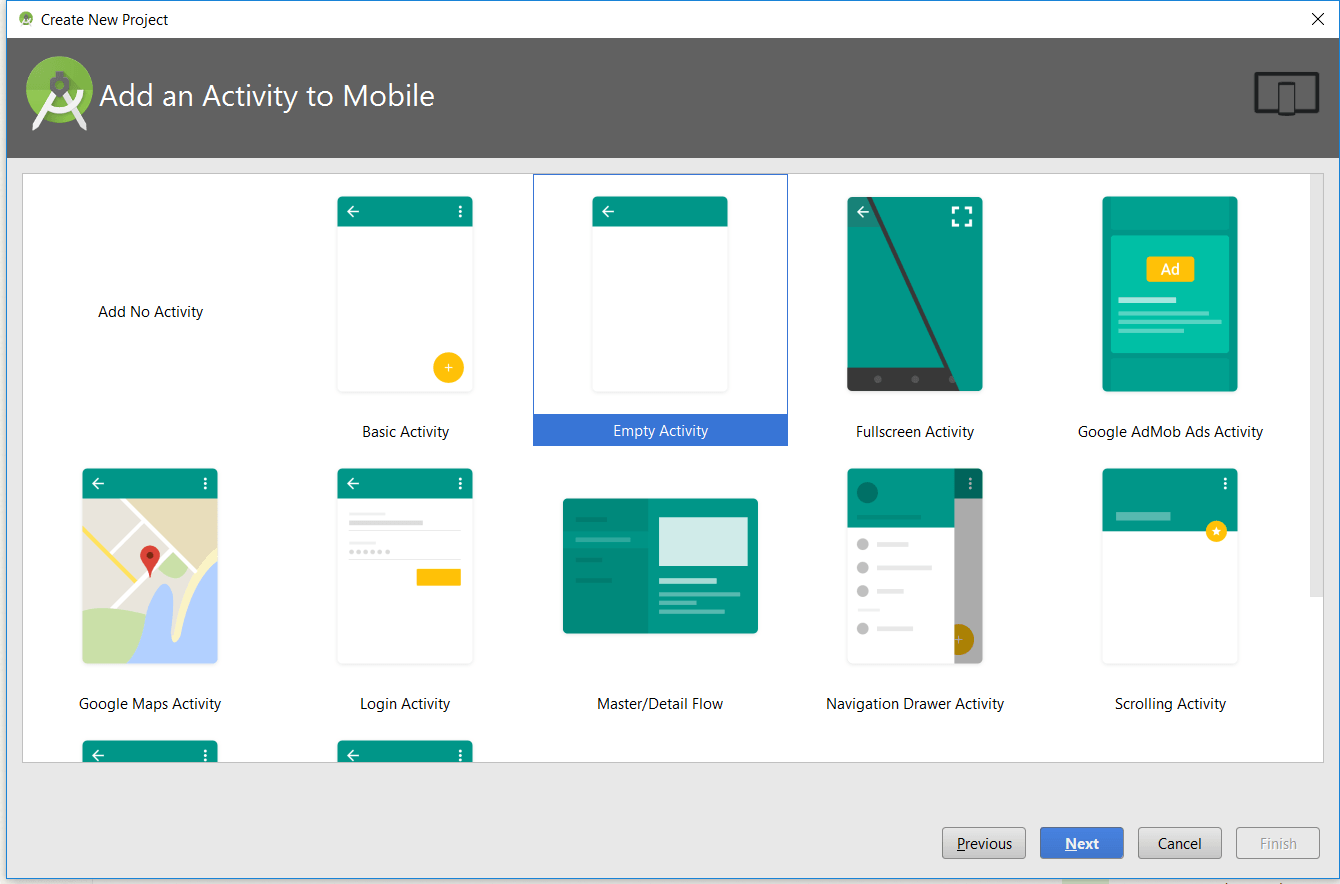
\includegraphics[width=\textwidth]{lab1-3}

\subsection{Choose name for the main activity. Choose default for now}

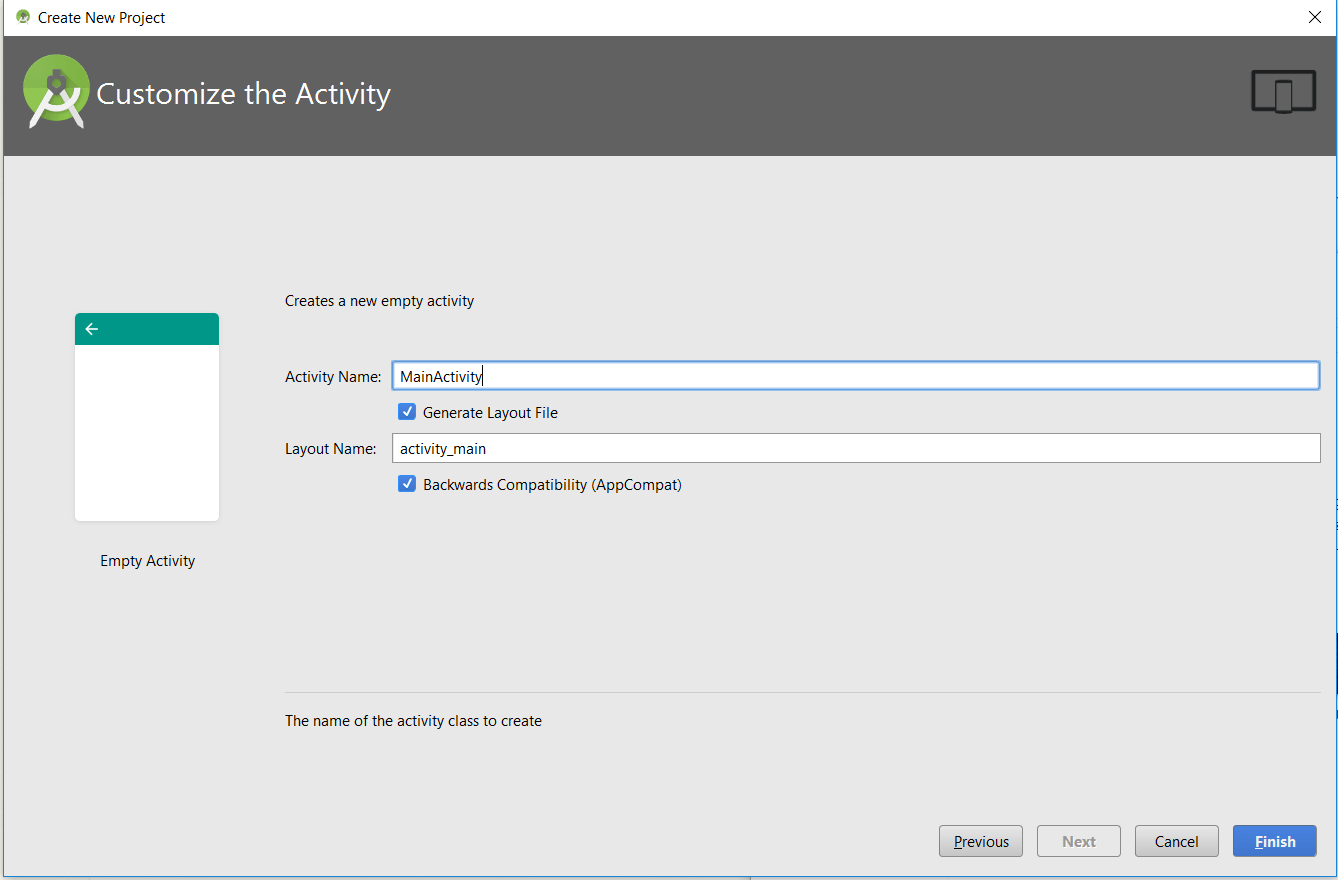
\includegraphics[width=\textwidth]{lab1-4}

\subsection{Click run project}

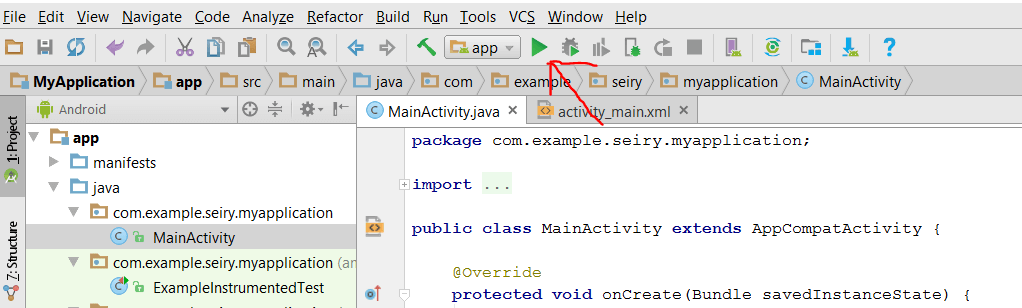
\includegraphics[width=\textwidth]{lab1-5}

\subsection{Choose target to run the application. You can connect your device with USB or create a virtual device}

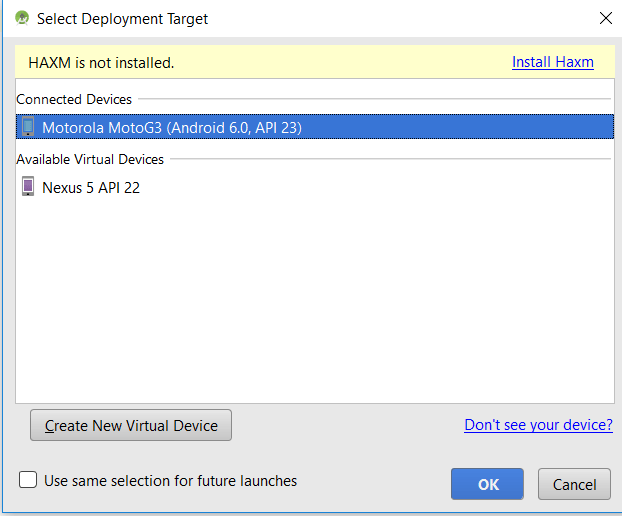
\includegraphics[width=\textwidth]{lab1-7}

\subsection{If you create a new device, you will be presented options to customize your virtual device, and download the necessary components}

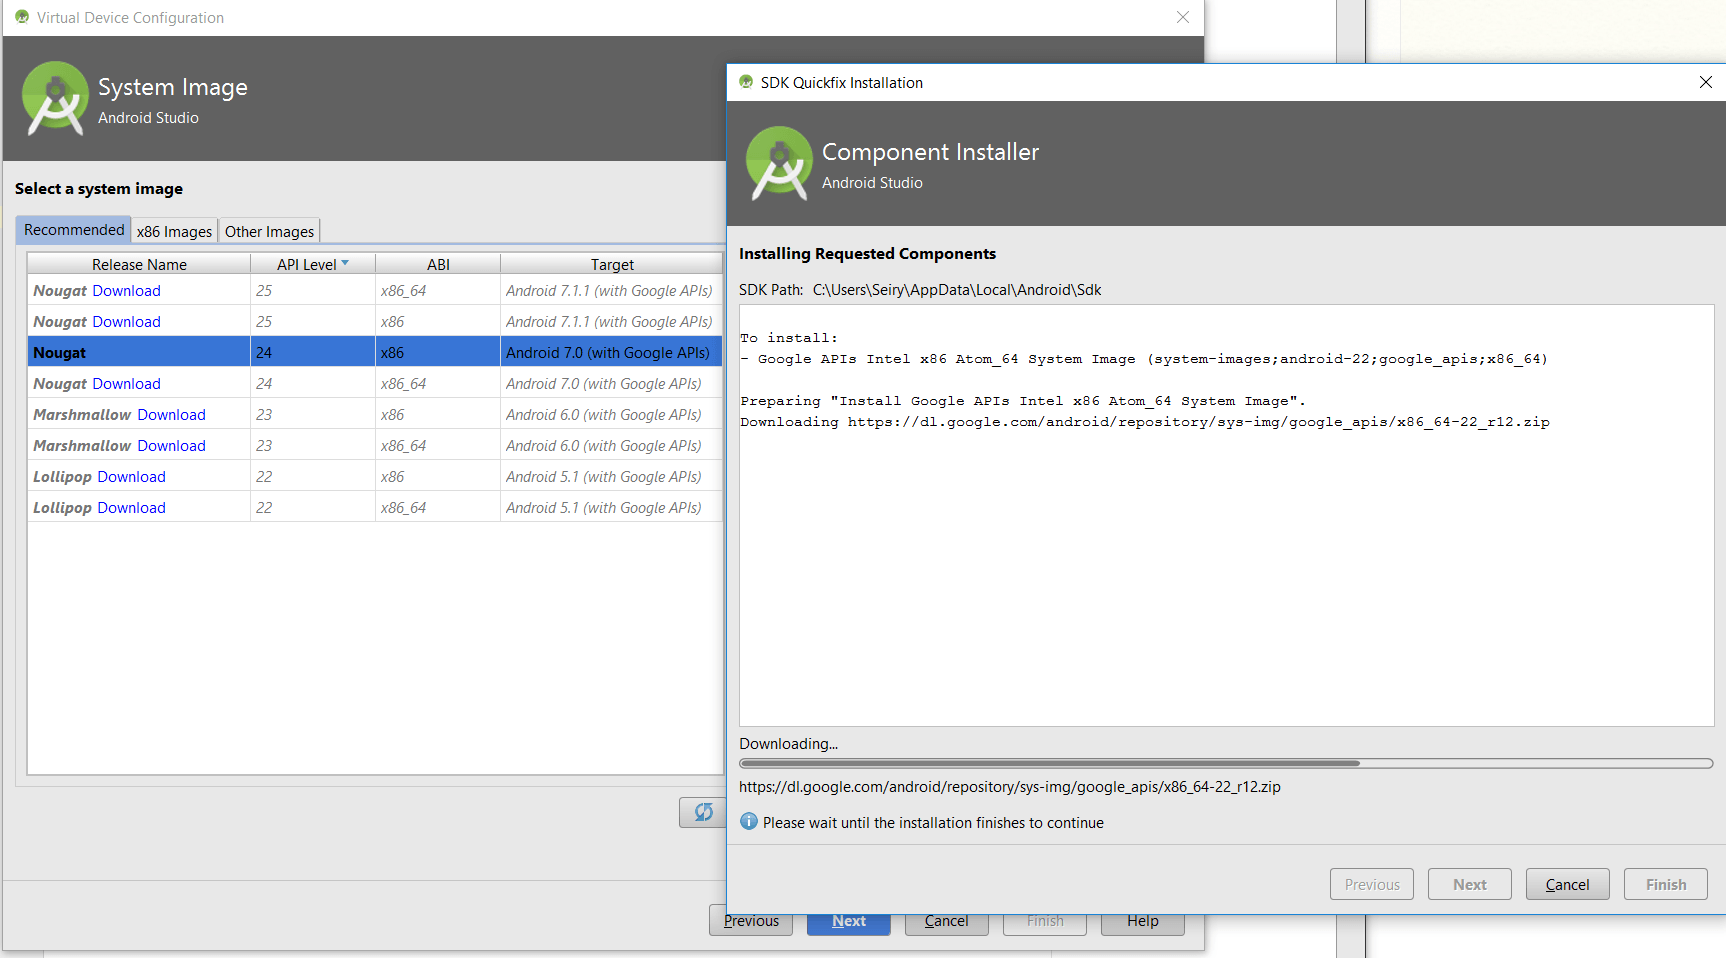
\includegraphics[width=\textwidth]{lab1-6}

\subsection{Click ok when done choosing your device target}

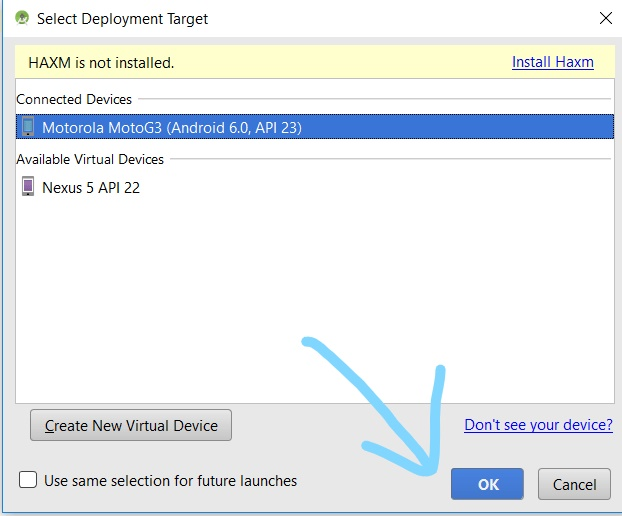
\includegraphics[width=\textwidth]{lab1-9}


\subsection{Your hello world application is ready}

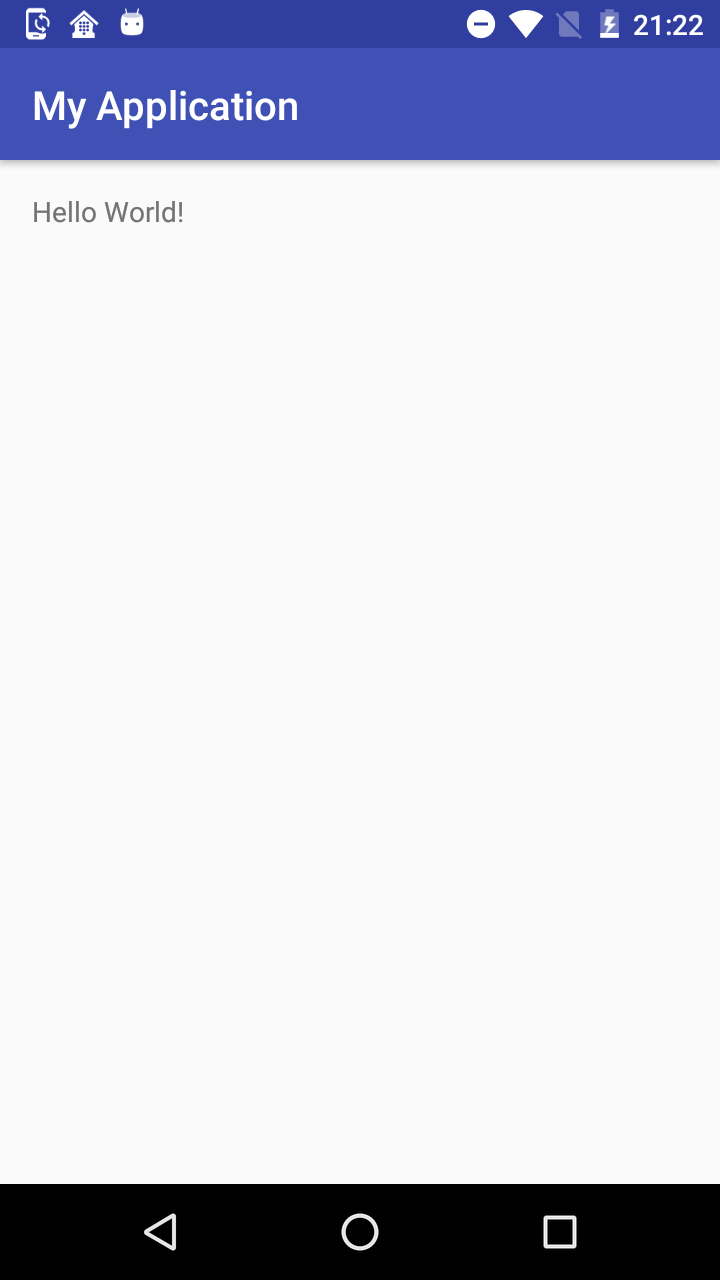
\includegraphics[width=\textwidth]{lab1-8}

\end{document}
